
\begin{figure*}
\resizebox{\linewidth}{!}{ % Automatically scales diagram to fit page width
\begin{tikzpicture}[
    function/.style={rectangle, draw, rounded corners, minimum width=2cm, minimum height=1cm, text centered, node distance=1.5cm},
    distribution/.style={ellipse, draw, minimum width=2cm, minimum height=1cm, text centered, node distance=1.2cm},
    gaussian/.style={draw, smooth, samples=100, domain=-2.5:2.5},
    snpk/.style={rectangle, draw, rounded corners, minimum width=2.5cm, minimum height=1cm, text centered, node distance=1.5cm, fill=blue!20},
    level 1/.style={sibling distance=6cm, level distance=2cm},
    level 2/.style={sibling distance=2cm, level distance=3cm},
    mss/.style={fill=red!50, draw=black},
    ploss/.style={fill=blue!50, draw=black},
    likert/.style={fill=green!40, draw=black}
]

% Existing functions and distributions diagram
\node[function] {Synthesizer Program}
    child { node[function] {DTW\_Onset}
        child { node[distribution, mss] {MSS}
            child[grow=down, level distance=1.5cm] {
                node[draw=none] {
                    \begin{tikzpicture}[scale=0.7]
                        \draw[red] plot (\x/3, {exp(-\x*\x)});  % Red Gaussian
                    \end{tikzpicture}
                }
            }
        }
        child { node[distribution, ploss] {P-Loss}
            child[grow=down, level distance=1.5cm] {
                node[draw=none] {
                    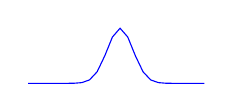
\begin{tikzpicture}[scale=0.7]
                        \draw[blue] plot (\x/3, {exp(-\x*\x)});  % Blue Gaussian
                    \end{tikzpicture}
                }
            }
        }
        child { node[distribution, likert] {Likert}
            child[grow=down, level distance=1.5cm] {
                node[draw=none] {
                    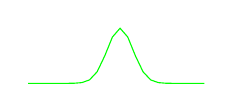
\begin{tikzpicture}[scale=0.7]
                        \draw[green] plot (\x/3, {exp(-\x*\x)});  % Green Gaussian
                    \end{tikzpicture}
                }
            }
        }
    }
    child { node[function] {L1\_Spec}
        child { node[distribution, mss] {MSS} }
        child { node[distribution, ploss] {P-Loss} }
        child { node[distribution, likert] {Likert} }
    }
    child { node[function] {SIMSE\_Spec}
        child { node[distribution, mss] {MSS} }
        child { node[distribution, ploss] {P-Loss} }
        child { node[distribution, likert] {Likert} }
    }
    child { node[function] {JTFS}
        child { node[distribution, mss] {MSS}
            child[grow=down, level distance=1.5cm] {
                node[draw=none] {
                    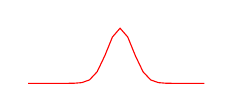
\begin{tikzpicture}[scale=0.7]
                        \draw[red] plot (\x/3, {exp(-\x*\x)});  % Red Gaussian
                    \end{tikzpicture}
                }
            }
        }
        child { node[distribution, ploss] {P-Loss}
            child[grow=down, level distance=1.5cm] {
                node[draw=none] {
                    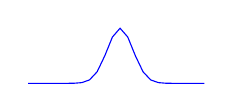
\begin{tikzpicture}[scale=0.7]
                        \draw[blue] plot (\x/3, {exp(-\x*\x)});  % Blue Gaussian
                    \end{tikzpicture}
                }
            }
        }
        child { node[distribution, likert] {Likert}
            child[grow=down, level distance=1.5cm] {
                node[draw=none] {
                    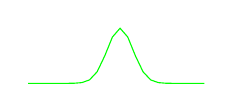
\begin{tikzpicture}[scale=0.7]
                        \draw[green] plot (\x/3, {exp(-\x*\x)});  % Green Gaussian
                    \end{tikzpicture}
                }
            }
        }
    };

% Label for the second row (Distributions)
\node at (0,-6.5) {\textbf{$\longleftarrow$\ \ \large Bootstrapped Distributions\ \ $\longrightarrow$}};

% Left side: SNPK with MSS
\node[snpk, text height=5ex, align=center, fill=red!30, draw=black] at (-6,-9) {SNPK with 4 \\ MSS distributions};
\draw[->] (-6,-9.5) -- (-6,-10.5) node[below, below] {\textbf{Ranks 1-4}};
\draw[red!40, thick] (-4.5, -8.4) -- (-2.75, -7.75);  % Line 1
\draw[red!40, thick] (-5.25, -8.4) -- (-3.5, -7.75);  % Line 2
\draw[red!40, thick] (-5.75, -8.4) -- (-5.5, -7.75);  % Line 3
\draw[red!40, thick] (-6.25, -8.4) -- (-9, -7.75);  % Line 4

% Middle: SNPK with P-Loss
\node[snpk, text height=5ex, align=center, fill=blue!40, draw=black] at (0,-9) {SNPK with 4 \\ P-Loss distributions};
\draw[->] (0,-9.5) -- (0,-10.5) node[below, below] {\textbf{Ranks 1-4}};
\draw[blue!40, thick] (1.5, -8.4) -- (3.25, -7.75);  % Line 1
\draw[blue!40, thick] (0.75, -8.4) -- (1.5, -7.75);  % Line 2
\draw[blue!40, thick] (-0.25, -8.4) -- (-1, -7.75);  % Line 3
\draw[blue!40, thick] (-0.75, -8.4) -- (-3, -7.75);  % Line 4

% Right side: SNPK with Likert
\node[snpk, text height=5ex, align=center, fill=green!30, draw=black] at (6,-9) {SNPK with 4 \\ Likert distributions};
\draw[->] (6,-9.5) -- (6,-10.5) node[below, below] {\textbf{Ranks 1-4}};
\draw[green!50, thick] (7.5, -8.4) -- (8.75, -7.75);  % Line 1
\draw[green!50, thick] (6.75, -8.4) -- (6, -7.75);    % Line 2
\draw[green!50, thick] (6.25, -8.4) -- (4, -7.75);   % Line 3
\draw[green!50, thick] (5.75, -8.4) -- (3, -7.75);     % Line 4

\end{tikzpicture}
}
\caption{For each synthesizer program, we assign ranks to the four loss functions  (\DTWEnv, \LoneSpec, \SIMSESpec, \JTFS) in three different ways, using MSS, P-Loss, or manually assigned Likert scores.}
\label{fig:posthoc_evaluation}
\end{figure*}